\subsection{Causal Inference: Train-test Split}
\label{Causal Inference: Train-test Split}

In section \ref{Covariate-level Topic Analysis}, we first estimated latent topic proportions using the STM and then assessed the relation between these document-level topic proportions and prevalence covariates. In particular, the documents that were used to obtain the topic proportions were the same that were subsequently used to quantify relationships between covariates and topic proportions. As \cite{egami2018make} argue, this double usage of data causes both an identification problem and an overfitting problem; hence inferences about covariate effects are biased. Additionally, since in the STM prevalence covariates affect estimated topic proportions, there is not only a double usage of data (i.e., in the sense that the same documents are used twice), but also a direct double usage of prevalence covariates as the estimated latent topic proportions are regressed on the former.

The problems arising from double usage of documents are best understood when considering a classical causal inference scenario. Therefore, assume that there are two groups, a treatment group and a control group. Aside from treatment, individuals from both groups are similar. The objective is to quantify the treatment effect, which in our case is the effect of treatment on the prevalence of a specific topic. The identification problem occurs because estimating the topic model in order to discover latent topic proportions can introduce an additional dependency among individuals. In such a case the response of an individual (i.e., the topic proportion) depends not only on treatment of this individual, but also on treatment of other individuals. Consequently, the estimation of treatment effects in the second stage is biased, since the assumption that the response is only determined by treatment of that individual is not valid. In addition to this identification problem, we might face an instance of overfitting: as with any model, we likely mistake noise for patterns. In such a case, again, the response is not solely determined by treatment of an individual, but additionally by specific characteristics of other individuals. This also results in a biased estimate of the treatment effect.

The problems described can be addressed using a framework proposed by \cite{egami2018make}. The general idea is to split the data $\mathcal{D}$ into a training set $\mathcal{D}_{\text{train}}$ and a test set $\mathcal{D}_{\text{test}}$. The training set is used to determine a model in order to infer latent topic proportions from any text assumed to be generated by the same underlying process as the training set. Subsequently, this estimated model is applied to the test set in order to assess the relation between test set topic proportions and test set prevalence covariates. The train-test split solves the identification problem, because when predicting the topic proportion for an individual on the test set, there is no dependence on treatment of other individuals from the test set since the model used for prediction is determined by training set observations only. Therefore, when estimating the treatment effect by comparing predicted proportions between different test set observations, the assumption that each proportion is independent of other \textit{test set} individuals' treatment holds. Likewise, idiosyncratic noise from the training set, which determines the model used to predict test set topic proportions, is unlikely to be found on the test set. Thus, the problem of overfitting is also solved. In the following, we explain the exact procedure for the STM (note that \cite{egami2018make} focus, for the most part, on the general framework, while the technical details of the implementation within the STM are not discussed in depth) and evaluate the results when applied to our data.

\subsubsection{Model Estimation on the Training Set}
\label{Model Estimation on the Training Set}

On the training set, we estimate components of the STM similarly to the estimation on the full data set. That is, we input documents, i.e., words and metadata from the training set, and obtain estimates $(\hat{\boldsymbol{\beta}}_{\text{train}}, \hat{\boldsymbol{\Gamma}}_{\text{train}}, \hat{\boldsymbol{\Sigma}}_{\text{train}})$, where $\hat{\boldsymbol{\beta}}_{\text{train}}$ is associated with the topic-word distribution and $\hat{\boldsymbol{\Gamma}}_{\text{train}}$ as well as $\hat{\boldsymbol{\Sigma}}_{\text{train}}$ are the topical prevalence parameters. 

\subsubsection{Prediction of Topic Proportions on the Test Set}
\label{Prediction of Topic Proportions on the Test Set}

Prediction of topic proportions on the test is not straightforward, since the topic proportions are latent and the STM was not designed for the specific purpose of predicting these latent variables on a set of new, unseen data. The fundamental idea is to estimate the variational posterior of the latent variables, that is, the topic proportions $\boldsymbol{\theta}_d$, where $d \in \mathcal{D}_{\text{test}}$ (note that $\boldsymbol{z}_d$ is integrated out in the STM), conditional on the model parameters $(\hat{\boldsymbol{\beta}}_{\text{train}}, \hat{\boldsymbol{\Gamma}}_{\text{train}}, \hat{\boldsymbol{\Sigma}}_{\text{train}})$ from the training set as well as the words $\boldsymbol{W}_{\text{test}}$ from the test set. This functionality is implemented in the \textit{stm} package through the function \textit{fitNewDocuments}, which by default outputs the MAP estimates of topic proportions $\boldsymbol{\theta}_d$, for all $d \in \mathcal{D}_{\text{test}}$. Note that estimating the variational posterior of the latent variables, conditioned on the parameters and the words, is precisesly what occurs during each E-step of the EM Algorithm. Thus, the implementation of \textit{fitNewDocuments} simply consists of one E-step with inputs $(\hat{\boldsymbol{\beta}}_{\text{train}}, \hat{\boldsymbol{\Gamma}}_{\text{train}}, \hat{\boldsymbol{\Sigma}}_{\text{train}}, \boldsymbol{W}_{\text{test}})$. It is, however, not obvious how to exactly input $\hat{\boldsymbol{\Gamma}}_{\text{train}}$ and  $\hat{\boldsymbol{\Sigma}}_{\text{train}}$ into the E-step. Depending on the characteristics of the specific analysis conducted by the researcher, \cite{egami2018make} propose three different alternatives:
\begin{enumerate}
\item \textbf{Covariate-specific prior}: Before applying the E-step, $\hat{\boldsymbol{\Gamma}}_{\text{train}}$ is used to obtain $\hat{\boldsymbol{\mu}}_d := (\hat{\boldsymbol{\Gamma}}_{\text{train}})^T(\boldsymbol{x}_d)^T$, for each document $d \in \mathcal{D}_{\text{test}}$ in the test set. Each document is then updated performing the E-step with inputs $(\boldsymbol{\mu}_d, \boldsymbol{\Sigma}, \boldsymbol{\beta}) = (\hat{\boldsymbol{\mu}}_d, \hat{\boldsymbol{\Sigma}}_{\text{train}}, \hat{\boldsymbol{\beta}}_{\text{train}})$ together with the respective document-specific words; for the exact update machanism see \cite{roberts2013structural}, pp. 992-993. The problem with this approach is, however, that for two documents from the test set containaing the exact same words, different topic proportions are predicted if the prevalence covariates differ. However, in such a case we would want the causal effect of the covariates on the topic proportions to be zero.
\item \textbf{Average prior}: The average prior circumvents the problem of the covariate-specific prior, as described above, by simply using - for each document in the test set - the average $\overline{\boldsymbol{\mu}}_{\text{train}} := \frac{1}{|\mathcal{D}_{\text{train}}|}\sum_{d \in \mathcal{D}_{\text{train}}} (\hat{\boldsymbol{\Gamma}}_{\text{train}})^T(\boldsymbol{x}_d)^T$ of all document-specific means from the training set. The covariance $\hat{\boldsymbol{\Sigma}}_{\text{train}}$ - which we now denote as $\overline{\boldsymbol{\Sigma}}_{\text{train}}$ - is recalculated based on the new average $\overline{\boldsymbol{\mu}}_{\text{train}}$ according to formula (11) on p.\ 993 in \cite{roberts2013structural}. The E-step for each document $d \in \mathcal{D}_{\text{test}}$ from the test set is accordingly performed with inputs $(\boldsymbol{\mu}_d, \boldsymbol{\Sigma}, \boldsymbol{\beta}) = (\overline{\boldsymbol{\mu}}_{\text{train}}, \overline{\boldsymbol{\Sigma}}_{\text{train}}, \hat{\boldsymbol{\beta}}_{\text{train}})$ together with the document-specific words. In this scenario, prevalence covariates from the test set have no influence at all on the prediction of test set topic proportions. 
\item \textbf{No prior}: If no prior is used, then for each document $d \in \mathcal{D}_{\text{test}}$ in the test set the E-step is performed using $\boldsymbol{\mu}_d=0$ and replacing $\hat{\boldsymbol{\Sigma}}_{\text{train}}$ with a diagonal covariance matrix with very large diagonals.
\end{enumerate}
The covariate-specific prior cannot be used in our case due to the problem described above, that is, different topic proportions being predicted for identically worded test set documents if their prevalence covariates differ. The option "no prior" can be useful if the metadata on the test set is believed to be linked differently to topics than is the case on the training set. In most cases the second option, "average prior", should provide the best trade-off, since in this case metadata from the training set is directly used to predict topic proportions, but the problem of the covariate-specific prior is solved. Note that consequently there is no double usage of covariates in this case.

\subsubsection{Estimation of the Average Treatment Effect}
\label{Estimation of the Average Treatment Effect}

Following \cite{egami2018make}, we define the Average Treatment Effect (ATE) on prevalence of topic $k$ as
\begin{align}
\text{ATE}_k := \mathbb{E}[\theta^{\text{[treatment]}}_{d,k} - \theta^{\text{[control]}}_{d,k}],
\end{align}
where $\theta^{\text{[treatment]}}_{d,k}$ and $\theta^{\text{[control]}}_{d,k}$ denote the topic proportions for the $d$-th document and $k$-th topic under treatment and control, respectively. (Note that for document $d$, we only observe \textit{either} $\theta^{\text{[treatment]}}_{d,k}$ \textit{or} $\theta^{\text{[control]}}_{d,k}$.) That is, we are interested in the average effect of treatment on topic proportion $k$ of an individual, assuming that this average effect is identical across all individuals. In other words, we assume the change in a topic proportion induced by treatment is a random variable with equal mean for all individuals. 

In order to estimate $\text{ATE}_k$, as reasoned above, it is crucial to separate the documents used for constructing the mechanism to discover latent topic proportions from the documents to which we apply this mechanism. Formally, using either the option "no prior" or "average prior", we can denote this mechanism as a function $g_{\text{train}}$, which we determine on the training data together with the parameters $(\hat{\boldsymbol{\beta}}_{\text{train}}, \hat{\boldsymbol{\Gamma}}_{\text{train}}, \hat{\boldsymbol{\Sigma}}_{\text{train}})$. The prediction of the $k$-th topic proportion for a test set observation $d \in \mathcal{D}_{\text{test}}$ (as outlined above) can then be written as $\hat{\theta}_{d,k} = g_{\text{train}}(\boldsymbol{w_d}, \hat{\boldsymbol{\beta}}_{\text{train}}, \hat{\boldsymbol{\Gamma}}_{\text{train}}, \hat{\boldsymbol{\Sigma}}_{\text{train}})$, where $\boldsymbol{w_d}$ denotes the observed words of document $d$. 

To estimate the treatment effect on a data set $\mathcal{D}$, we determine the average difference of predicted topic proportions between both groups, i.e.,
\begin{align}
\widehat{\text{ATE}_k} = \frac{1}{|\mathcal{D}_{\text{treatment}}|}\sum_{d \in \mathcal{D}_{\text{treatment}}} \hat{\theta}_{d,k} - \frac{1}{|\mathcal{D}_{\text{control}}|}\sum_{d \in \mathcal{D}_{\text{control}}} \hat{\theta}_{d,k},
\end{align} 
where $\hat{\theta}_{d,k}$ is the predicted topic proportion for the $d$-th document and $k$-th topic. \cite{egami2018make} show that, if additional conditions hold, $\widehat{\text{ATE}_k}$ estimated on previously unseen test data $\mathcal{D}_{\text{test}}$ is an unbiased estimate of $\text{ATE}_k$.\footnote{Precisely, we predict $\hat{\theta}_{d,k} = g_{\text{train}}(\boldsymbol{w_d}, \hat{\boldsymbol{\beta}}_{\text{train}}, \hat{\boldsymbol{\Gamma}}_{\text{train}}, \hat{\boldsymbol{\Sigma}}_{\text{train}})$, for each document $d \in \mathcal{D}_{\text{test}}$.}
In contrast, if we do not split the data and "na{\"i}vely" predict topic proportions on the same data used to estimate the topic model, we obtain a biased estimate, due to both the identification problem and the overfitting problem described above.

\subsubsection{Results}
\label{Results}

We now depict our results from the train-test split, where we split the data into two equally sized sets, for the options "average prior" and "no prior". Note that the test data cannot consist of words which have not been seen in the training data. Therefore, all previously unseen words are removed from the test data. After removing the words, the test data contains 80.6\% of the original words. Since we use only a subset of the full data, the estimated topics are slightly different from those obtained using the full data; however, most topics are similar. We assign new labels to the topics, a complete list of which can be found in the accompanying R code of this paper.

In contrast to section \ref{Covariate-level Topic Analysis}, the focus of this section lies on quantifying causal effects between covariates and the relevance of a topic, since the train-test framework is most appropriate to conduct such types of analyses. As mentioned before, \textit{fitNewDocuments} outputs the MAP estimates of the variational posterior of topic proportions for the test set. In Figure \ref{fig:causal_inference_props} we depict these MAP estimates of topic proportions, along with topic proportions obtained for the training data, for two selected topics.

The UN Climate Action Summit 2019 was held on September 23, 2019. As can be observed in the left panel of Figure \ref{fig:causal_inference_props} below, the topic associated with climate issues was discussed to a much larger extent during that time than the year before. While the MAP estimates for the different prior specifications on the test set are rather similar, the estimated effect for the training data is much larger. If we compare the estimated topic proportions for a topic we labelled as 'Emancipation' for the two opposing parties 'AfD' and 'B{\"u}ndnis 90/Die Gr{\"u}nen', we find similar results (see right panel of Figure \ref{fig:causal_inference_props}): the average difference of estimated topic proportions between both parties is larger on the training data. Also, note that credible intervals on the training data differ from those on the test data in both cases.

\begin{figure}[h!]
  \centering
  \captionsetup{justification=centering}
  \begin{subfigure}[b]{0.49\linewidth}
    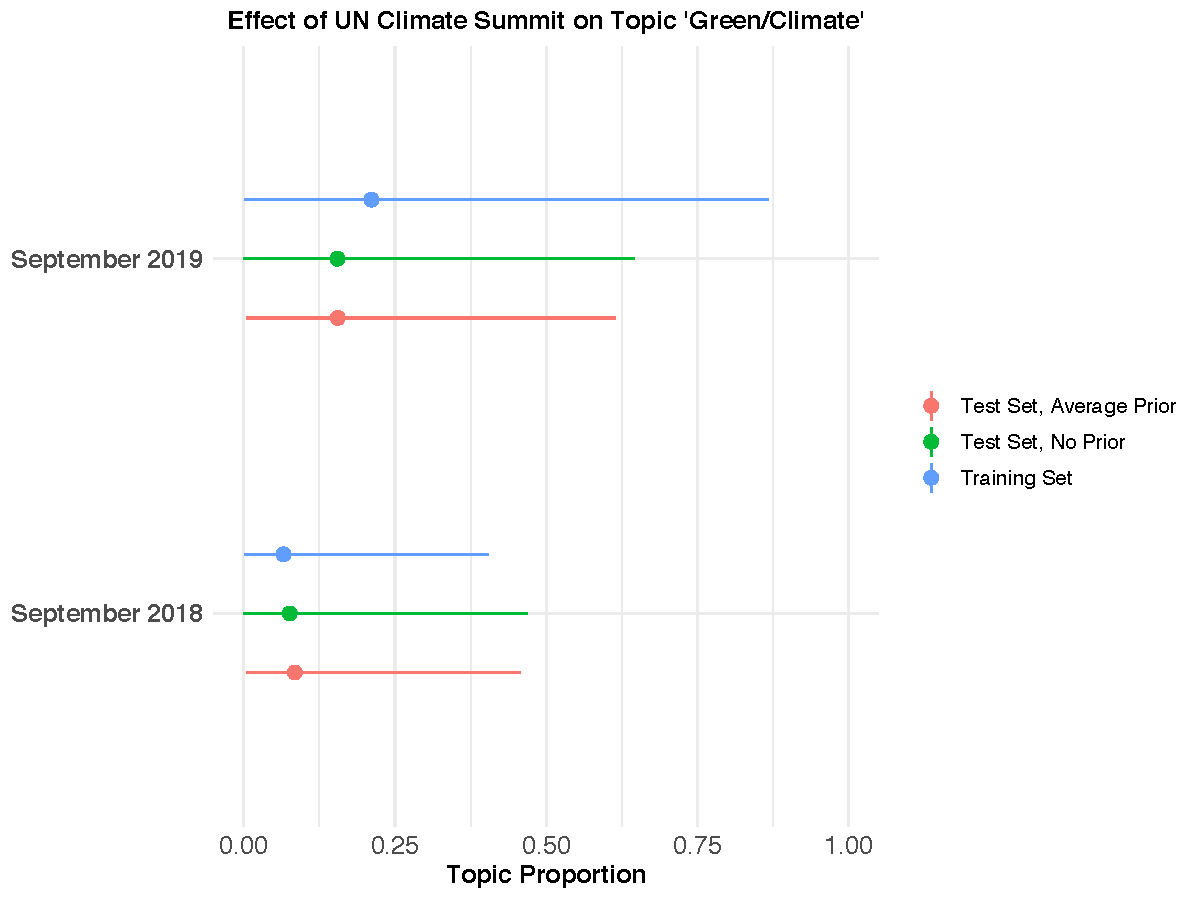
\includegraphics[width=\linewidth]{../plots/6_2/climate_summit_props.pdf}
  \end{subfigure}
  \begin{subfigure}[b]{0.49\linewidth}
    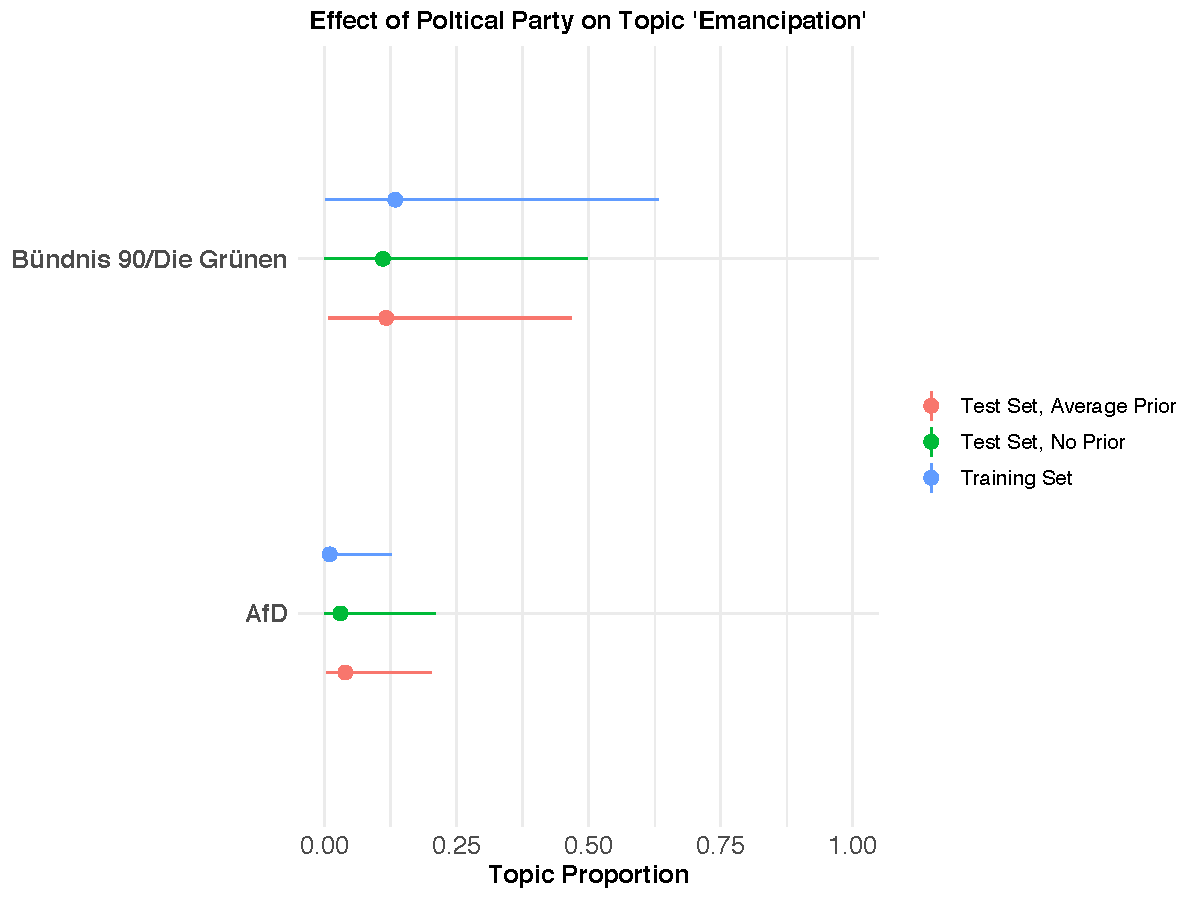
\includegraphics[width=\linewidth]{../plots/6_2/emancipation_props.pdf}
  \end{subfigure}
  \caption{Maximum-a-posteriori (MAP) estimates of topic proportions on training and test data. Points display the mean, lines 2.5\% and 97.5\% credible intervals.}
  \label{fig:causal_inference_props}
\end{figure}

In Figure \ref{fig:causal_inference_ate} we visualize the ATE estimated on training and test data with different prior specifications (note that this is simply the difference of the means depicted in Figure \ref{fig:causal_inference_props}). The results confirm that there is a substantial difference between the estimated effects.

\begin{figure}[h!]
  \centering
  \captionsetup{justification=centering,margin=2cm}
  \begin{subfigure}[b]{0.49\linewidth}
    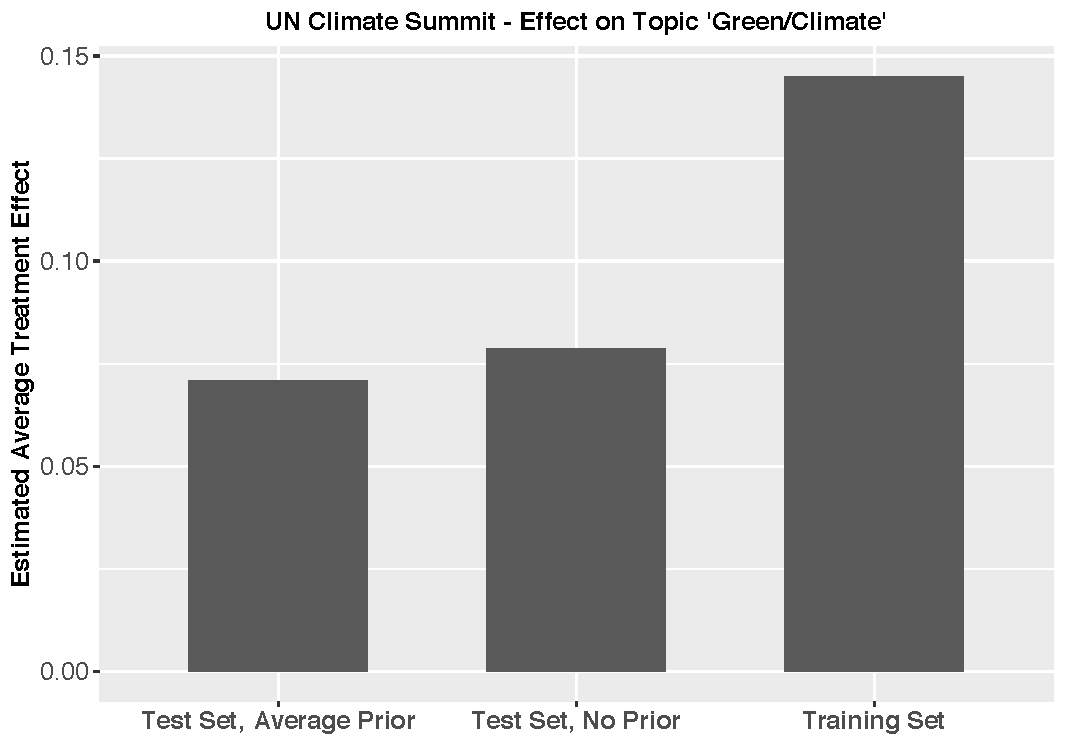
\includegraphics[width=\linewidth]{../plots/6_2/climate_summit_ate.pdf}
  \end{subfigure}
  \begin{subfigure}[b]{0.49\linewidth}
    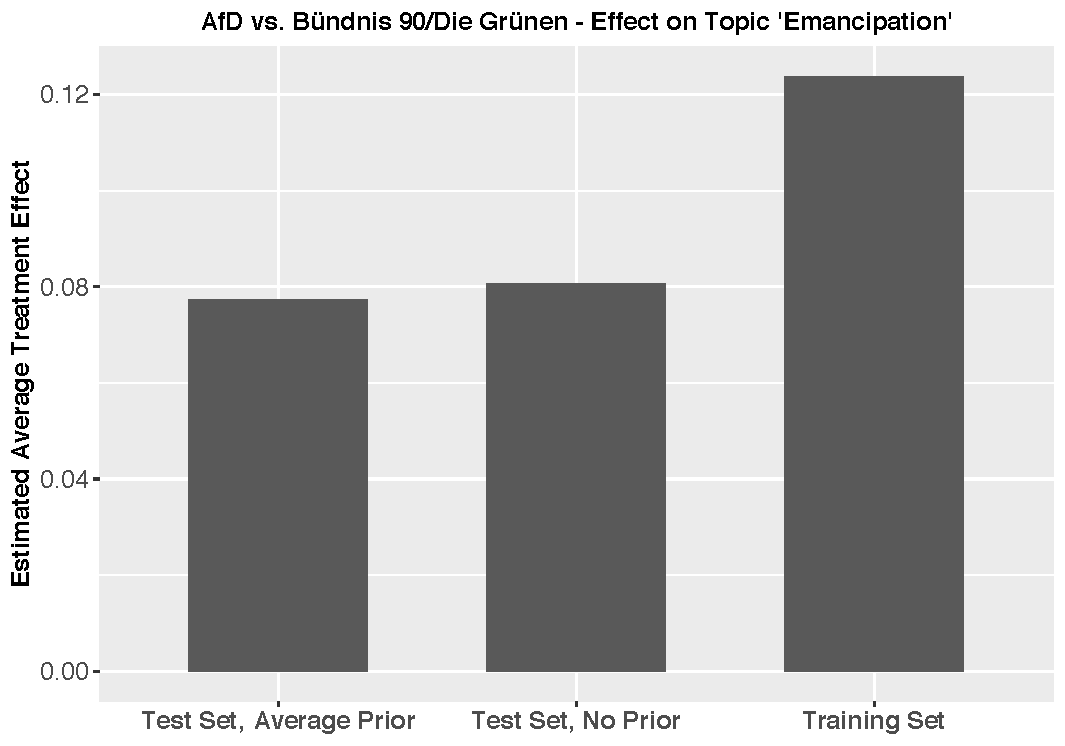
\includegraphics[width=\linewidth]{../plots/6_2/emancipation_ate.pdf}
  \end{subfigure}
  \caption{Estimated Average Treatment Effects (ATE) using training and test data.}
  \label{fig:causal_inference_ate}
\end{figure}

Finally, note that there are several general concerns when conducting a causal inference study. For instance, if the treatment group is not a random subsample of the population, the resulting estimator of the treatment effect might suffer from selection bias.